In \autoref{sec:rings} we defined a kind of abstract structure, called a \emph{ring}, which generalizes the arithmetic of the integers.
We also gave a list of several examples which will be amended as we move along.
To help us make sense of a growing menagerie of rings we now introduce some useful special properties that a ring may or may not possess.

\begin{dfn} \label{dfn:ring-fams}
Let \(R\) be a ring.
We say that \(R\) is \emph{commutative} \index{ring!commutative} if it satisfies the following property C (otherwise \(R\) is \emph{noncommutative}).
\begin{proplist}
\item[C.] \(ab = ba\) for all \(a,b \in R\).
\end{proplist}
We say that \(R\) is \emph{unital} \index{unital!ring} if it satisfies the following property U (otherwise \(R\) is \emph{nonunital}).
\begin{proplist}
\item[U.] There is an element \(1_R \in R\) (called a \emph{one}), different from \(0_R\), such that \(1_R \cdot a = a \cdot 1_R = a\) for all \(a \in R\).
\end{proplist}
We say that \(R\) is \emph{finite} if the set \(R\) has finite cardinality (otherwise \(R\) is \emph{infinite}).
\end{dfn}

Just as the zero element of a ring is not literally the number zero, a one in a ring is not literally the number one, but rather a distinguished element that \emph{acts like} one.

Any given ring can have any combination of these properties.
Many of the rings we are used to, such as \(\ZZ\), are commutative and unital.
In fact many rings which are useful in practice are both commutative and unital, and so in this text we will refer to such rings as \emph{CU rings}\index{ring!CU}.
However it is important to remember that there are plenty of interesting rings which are not commutative or not unital.

\begin{examples}
\item The number rings \(\ZZ\), \(\ZZ/(n)\), \(\QQ\), \(\RR\), and \(\CC\) are all both commutative and unital.
Of these, only \(\ZZ/(n)\) is finite, when \(n > 0\).

\item If \(R\) is unital then \(\MAT{2}{R}\) is also unital, with \[ 1_{\MAT{2}{R}} = \begin{bmatrix} 1_R & 0_R \\ 0_R & 1_R \end{bmatrix}. \]
Is this ring ever commutative?
Is it ever finite?

\item If \(R\) is unital, then (like every other element of $R$) the element \(1_R\) has a unique negative, called \(-1_R\).
These two elements need not be distinct!
For example in \(\ZZ/(2)\) we have \(1 = -1\) since \(1 + 1 = 2 \equiv 0\).

\item The ring \(2\ZZ\) of even integers is \emph{not} unital.
Why?
\end{examples}

As we might expect, some of the nice properties of the integer 1 are shared by the one element of any ring.

\begin{prop}
Let \(R\) be a unital ring.
\begin{proplist*}
\item The one element of \(R\) is unique in the following sense: if \(u \in R\) such that \(u \cdot a = a\) for all \(a \in R\), then \(u = 1_R\).
\item \((-1_R) \cdot a = -a\) for all \(a \in R\).
\end{proplist*}
\end{prop}

\begin{proof}
\begin{inlineproplist}
\item Suppose \(u\) is such an element; then we have \(1_R = u \cdot 1_R = u\).
\item Let \(a \in R\).
Then \(a + (-1_R)a = 1_R a + (-1_R)a = (1_R + (-1_R))a = 0a = 0\), so that \((-1_R)a = -a\) by \sref{prop:ring-basics}{negative-unique}.
\end{inlineproplist}
\end{proof}

If a ring is finite and small enough we can visualize its structure using two \emph{cayley tables}\index{cayley table} - one for plus and one for times.
These are simply addition and multiplication tables like the ones elementary school students learn, with the arithmetic done in \(R\) rather than in \(\ZZ\).
For example, the cayley tables of \(\ZZ/(5)\) are shown in \autoref{fig:cayley-zz5}.
The entry in row \(a\) and column \(b\) is \(a+b\) in the addition table and is \(ab\) in the multiplication table.
(It is important to keep this convention straight if \(R\) happens to be noncommutative!)
\begin{figure}[h!]
\begin{center}
\begin{tabular}{c|ccccc}
\(+\)
  & 0 & 1 & 2 & 3 & 4 \\ \hline
0 & 0 & 1 & 2 & 3 & 4 \\
1 & 1 & 2 & 3 & 4 & 0 \\
2 & 2 & 3 & 4 & 0 & 1 \\
3 & 3 & 4 & 0 & 1 & 2 \\
4 & 4 & 0 & 1 & 2 & 3
\end{tabular}
\quad\quad
\begin{tabular}{c|ccccc}
\(\cdot\)
  & 0 & 1 & 2 & 3 & 4 \\ \hline
0 & 0 & 0 & 0 & 0 & 0 \\
1 & 0 & 1 & 2 & 3 & 4 \\
2 & 0 & 2 & 4 & 1 & 3 \\
3 & 0 & 3 & 1 & 4 & 2 \\
4 & 0 & 4 & 3 & 2 & 1
\end{tabular}
\caption{\label{fig:cayley-zz5} Cayley tables of \(\ZZ/(5)\).}
\end{center}
\end{figure}
Cayley tables quickly become unwieldy as the size of a ring increases.
However if a ring is small enough its cayley tables give us a nice way to ``see'' some important concepts.
For instance, the defining property of zero is reflected in the row and column of zero in the additive cayley table, and similarly for one in the multiplicative table.
\begin{figure}[h!]
\small
\begin{center}
\begin{tabular}{c|cccccccc}
\(+\) & -   & a   & b   & c   & ab  & ac  & bc  & abc \\ \hline
-     & -   & a   & b   & c   & ab  & ac  & bc  & abc \\
a     & a   & -   & ab  & ac  & b   & c   & abc & bc  \\
b     & b   & ab  & -   & bc  & a   & abc & c   & ac  \\
c     & c   & ac  & bc  & -   & abc & a   & b   & ab  \\
ab    & ab  & b   & a   & abc & -   & bc  & ac  & c   \\
ac    & ac  & c   & abc & a   & bc  & -   & ab  & b   \\
bc    & bc  & abc & c   & b   & ac  & ab  & -   & a   \\
abc   & abc & bc  & ac  & ab  & c   & b   & a   & -
\end{tabular}

\medskip\medskip

\begin{tabular}{c|cccccccc}
\(\cdot\) 
    & -   & a   & b   & c   & ab  & ac  & bc  & abc \\ \hline
-   & -   & -   & -   & -   & -   & -   & -   & -   \\
a   & -   & a   & -   & -   & a   & a   & -   & a   \\
b   & -   & -   & b   & -   & b   & -   & b   & b   \\
c   & -   & -   & -   & c   & -   & c   & c   & c   \\
ab  & -   & a   & b   & -   & ab  & a   & b   & ab  \\
ac  & -   & a   & -   & c   & a   & ac  & c   & ac  \\
bc  & -   & -   & b   & c   & b   & c   & bc  & bc  \\
abc & -   & a   & b   & c   & ab  & ac  & bc  & abc
\end{tabular}
\caption{\label{fig:cayley-pow3} Cayley tables of \(\POW{\{a,b,c\}}\).}
\end{center}
\end{figure}
As another example, \autoref{fig:cayley-pow3} gives the cayley tables of \(\POW{\{a,b,c\}}\), with \(\varnothing\) denoted by a dash.
The fact that this ring is boolean is reflected in the main diagonal of the multiplication table, and that the characteristic is 2 is reflected in the main diagonal of the addition table.
Both \(\ZZ(5)\) and \(\POW{\{a,b,c\}}\) are commutative, which we can see because their multiplication tables are symmetric about the main diagonal.
Also, note that the multiplication table of \(\POW{\{a,b,c\}}\) has lots of zeros, but that of \(\ZZ/(5)\) only has zeros in the zero row and column.

Commutativity, finiteness, and the existence of a one are just three of many properties we will use to understand the different kinds of rings.
\autoref{fig:ring-venn} shows these families as a Venn diagram with examples in each region.
\begin{figure}[h]
\begin{center}
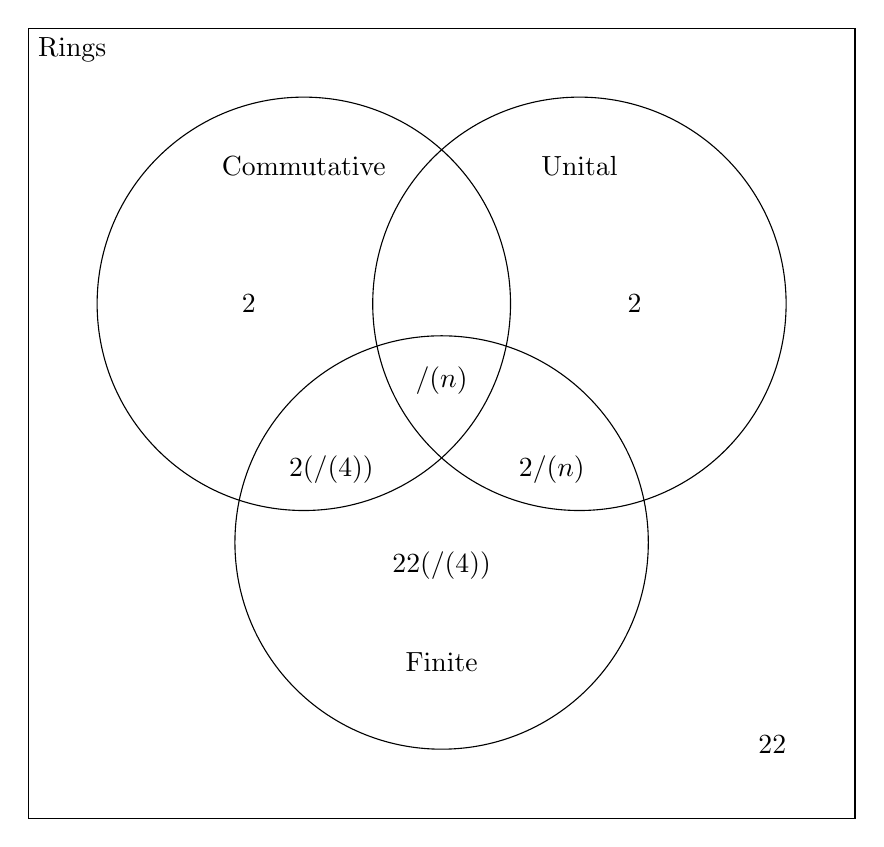
\begin{tikzpicture}[scale=0.35]
  \draw (-15,-18.66) -- (-15,10) -- (15,10) -- (15,-18.66) -- cycle;
  \draw (-5,0) circle (7.5);
  \draw (5,0) circle (7.5);
  \draw (0,-8.66) circle (7.5);
  \draw (-15,10) node [anchor=north west] {Rings};
  \draw (-5,5) node [anchor=center] {Commutative};
  \draw (5,5) node [anchor=center] {Unital};
  \draw (0,-13) node [anchor=center] {Finite};
  \draw (0,2.5) node [anchor=center] {\(\ZZ\)};
  \draw (0,-2.8) node [anchor=center] {\(\ZZ/(n)\)};
  \draw (-7,0) node [anchor=center] {\(2\ZZ\)};
  \draw (7,0) node [anchor=center] {\(\MAT{2}{\ZZ}\)};
  \draw (12,-16) node [anchor=center] {\(\MAT{2}{2\ZZ}\)};
  \draw (4,-6) node [anchor=center] {\(\MAT{2}{\ZZ/(n)}\)};
  \draw (-4,-6) node [anchor=center] {\(2(\ZZ/(4))\)};
  \draw (0,-9.5) node [anchor=center] {\(\MAT{2}{2(\ZZ/(4))}\)};
\end{tikzpicture}
\caption{\label{fig:ring-venn} A Venn diagram of ring families.}
\end{center}
\end{figure}



%---------%
\Exercises%
%---------%

\begin{exercise}
Show that \(\ZZ/(n)\) is a finite, commutative, unital ring for all \(n \geq 2\).
\end{exercise}


\begin{exercise}
Let \(X\) be a nonempty set.
\begin{proplist*}
\item Show that \(\POW{X}\) is commutative and unital, and that \(\POW{X}\) is finite if and only if \(X\) is finite.
\item Show that \(\POWP{X}\) is commutative and \emph{not} unital, and that \(\POWP{X}\) is finite if and only if \(X\) is finite.
\end{proplist*}
\end{exercise}


\begin{exercise}
Draw the cayley tables of the following rings.
This will be tedious.
\begin{proplist*}
\item \(\ZZ/(7)\)
\item \(\POWP{\{a,b\}}\)
\item \(\ZZ/(8)\)
\item \(\POW{\{a,b\}}\)
\item \(aR\), where \(R = \ZZ/(4)\) and \(a = [2]\)
\end{proplist*}
\end{exercise}


\begin{exercise}
Let \(R\) be a ring.
\begin{proplist}
\item Show that \(\MAT{2}{R}\) is unital if and only if \(R\) is unital.
\item Show that \(\MAT{2}{R}\) is finite if and only if \(R\) is finite.
\item Show that if \(R\) is not the zero ring, then \(\MAT{2}{R}\) is not commutative.
(Hint: find two specific matrices \(A\) and \(B\) such that \(AB \neq BA\).)
\end{proplist}
\end{exercise}


\begin{exercise}
Let \(R\) be a ring and \(A\) a nonempty set.
\begin{proplist}
\item Show that \(R^A\) is commutative if and only if \(R\) is commutative.
\item Show that \(R^A\) is unital if and only if \(R\) is unital.
\end{proplist}
\end{exercise}

\begin{exercise}
Show that the ring \(k\ZZ\), with \(k \geq 2\), is a commutative ring which is not unital.
(cf. \eref{exerc:aR-is-ring}.)
\end{exercise}


\begin{exercise}
If \(R\) is a unital ring, we can extend the power function \(a^\ast\) (cf. \ref{dfn:pow-elt}) to zero exponents by defining \(a^0 = 1_R\).
Show that if \(R\) is a unital ring, then the following properties hold for all \(a \in R\) and \(m,n \in \NN\).
\begin{proplist*}
\item \(a^{m+n} = a^m a^n\).
\item \(a^{mn} = (a^m)^n\).
\end{proplist*}
\end{exercise}


\begin{exercise}
Show that if \(R\) is commutative, then \((ab)^n = a^n b^n\) for all \(a,b \in R\) and all \(n \geq 1\).
If \(R\) is unital, show that this identity also holds for the case \(n = 0\).
\end{exercise}


\begin{exercise}[Binomial Theorem.] \label{exerc:binomial-theorem}
Let \(R\) be a commutative ring and let \(a,b \in R\).
Show that for all natural numbers \(n \geq 1\) we have \[ (a+b)^n = \sum_{k=0}^n {n \choose k} a^k b^{n-k}. \]
If \(R\) is unital, show that this identity also holds for the case \(n = 0\).
\end{exercise}


\begin{exercise}
Let \(R\) be a unital ring.
\begin{proplist*}
\item Suppose \(n1_R = 0_R\) for some \(n \geq 2\).
Show that \(\CHAR{R}\) divides \(n\).
\item Show that \(\CHAR{R} = \ADDORD{1_R}\).
\end{proplist*}
\end{exercise}


\begin{exercise}
Show that every finite ring has positive characteristic.
\end{exercise}


\begin{exercise}
Let \(R\) be a null ring.
\begin{proplist*}
\item Show that \(R\) is commutative.
\item Show that \(R\) is not unital.
\end{proplist*}
\end{exercise}


\begin{exercise}
Show that every boolean ring is commutative.
(Hint: Meditate upon \((a+b)^2\).)
\end{exercise}


\begin{exercise}
Exhibit a boolean ring which is unital, and another which is not unital.
\end{exercise}
